\section{Descriptivas}
\begin{table}[ht!]
        \centering
        \caption{Estadísticas descriptivas}
        \footnotesize{
        \begin{tabular}{l ccc c}\hline \hline
                &\multicolumn{1}{c}{Total}&\multicolumn{1}{c}{Masculinos}&\multicolumn{1}{c}{Femeninos}&\multicolumn{1}{c}{Dif (2)-(3)}\\\hline
                &\multicolumn{1}{c}{(1)}&\multicolumn{1}{c}{(2)}&\multicolumn{1}{c}{(3)}&\multicolumn{1}{c}{(4)}\\
            Edad      &    20.15&    20.25&    20.05&     0.20         \\
                            &  (1.710)&  (1.832)&  (1.589)&  [0.324]         \\
            Bogotá=1          &     0.59&     0.66&     0.52&     0.14         \\
                            &  (0.494)&  (0.478)&  (0.504)&  [0.093]         \\
            Semestres &     6.18&     5.96&     6.39&    -0.43         \\
                            &  (2.935)&  (3.057)&  (2.820)&  [0.556]         \\
            Apoyo financiero&     0.68&     0.61&     0.75&    -0.14         \\
                            &  (0.469)&  (0.493)&  (0.437)&  [0.088]         \\
                             &          &       &           &               \\
            Observaciones    &      112&       56&       56&      112         \\\hline \hline

        \end{tabular}}
        \begin{threeparttable} 
        \begin{tablenotes}
        \footnotesize{
        \item \textit{Nota}: Estadísticas descriptivas de los participantes del experimento. Desviaciones estándar en paréntesis. Errores estándares en corchetes; *** p$<$0.01, ** p$<$0.05, * p$<$0.1.}
        \end{tablenotes}
        \end{threeparttable}
    \end{table}

\subsection{Validación de norma social de habilidad}
\FloatBarrier 
\begin{figure}[ht!]
    \centering
    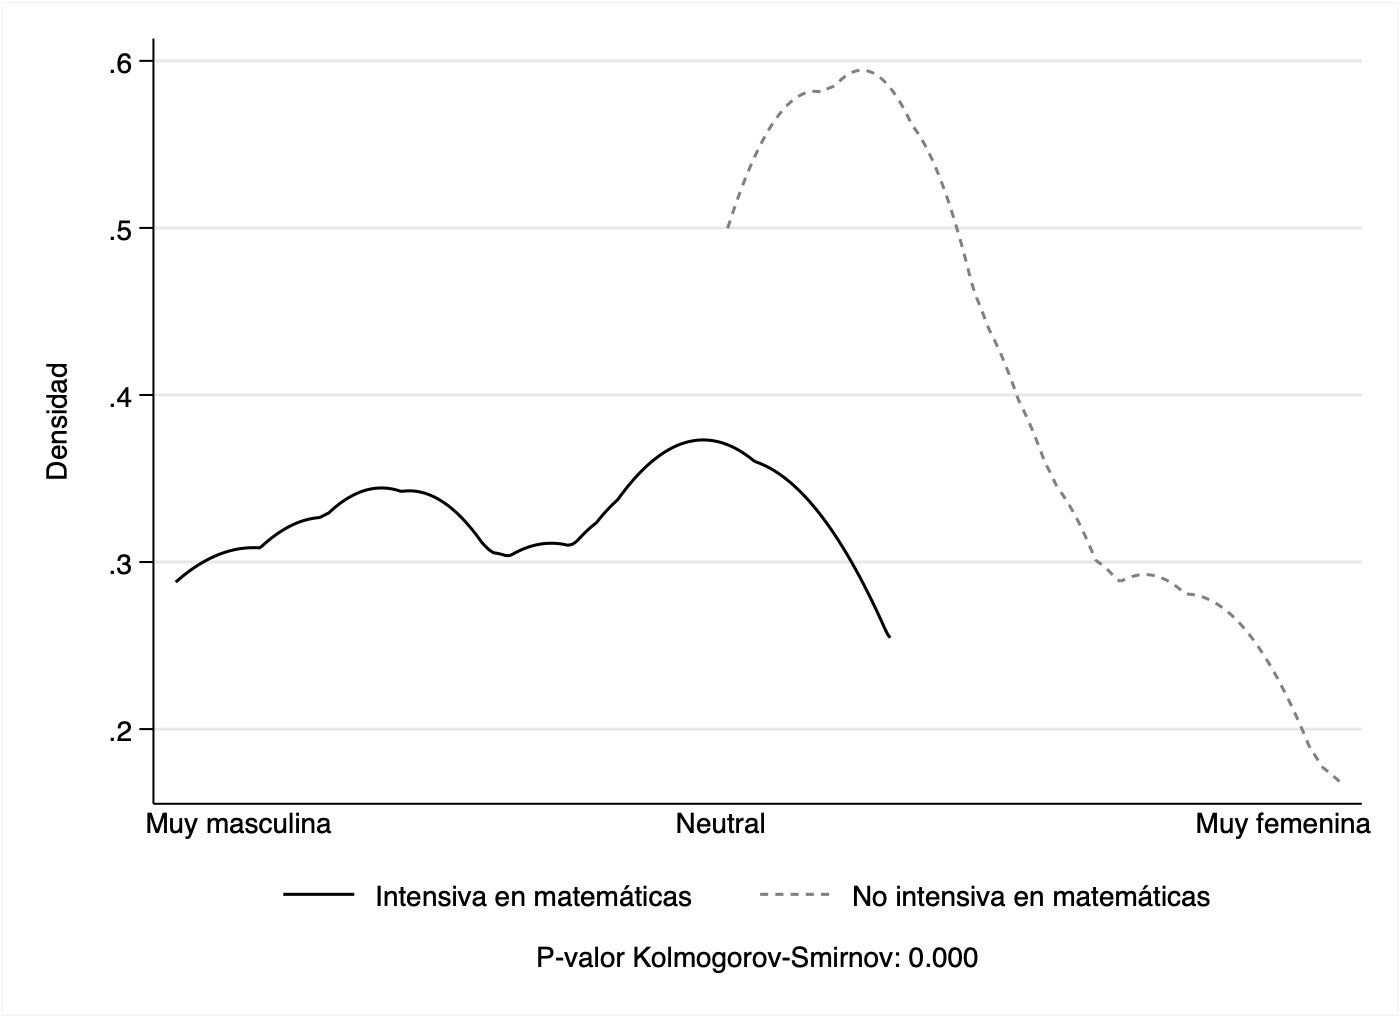
\includegraphics[width=12cm]{Images/career_perception.png}
    \caption{Percepción de carreras}
    \label{fig:careers}
    \begin{singlespace}
    \floatfoot{\footnotesize{\textit{Nota:} Gráfica de la percepción de 30 carreras clasificadas de 1 a 9 de muy masculina a muy femenina. La clasificación promedio hecha por una muestra de estudiantes, diferentes a los participantes del experimento. Las carreras son clasificadas como intensivas en matemáticas si tienen dos o más clases de matemáticas en su pensum, y como no intensivas de lo contrario.}\par}
    \end{singlespace}
\end{figure}


\subsection{Distribución de expresiones de género}
\FloatBarrier 
\begin{table}[ht]
    \centering
    \caption{Distribución por género de vestimenta, habilidades y aspiraciones}
    \label{tab:distribuciones_expresiones}
    \begin{subtable}{\textwidth}
        \centering
        \caption{Identidad masculina}
        \vspace*{-0.5cm}
        \fontsize{9.5}{12}\selectfont {
        \begin{tabular}{cccccc} \\ \hline \hline
                                & \multicolumn{2}{c}{Puntaje vestimenta $<$ 0} & & \multicolumn{2}{c}{Puntaje vestimenta $>$ 0} \\\cmidrule{2-3} \cmidrule{5-6}
                                & \textit{Económica}  & \textit{Familiar}      & &  \textit{Económica} & \textit{Familiar}      \\
        \textit{Matemáticas}    & 15                  & 11                     & & 1                   & 1                      \\
        \textit{Comunicación}   & 15                  & 11                     & & 1                   & 1                      \\\hline \hline
        \end{tabular}}
    \end{subtable}
    \begin{minipage}{\textwidth}
    \hspace*{2cm}
    \end{minipage}
    \begin{subtable}{\textwidth}
        \centering
        \vspace*{0.5cm}
        \caption{Identidad femenina}
        \vspace*{-0.5cm}
        \fontsize{9.5}{12}\selectfont {
        \begin{tabular}{cccccc}\\ \hline \hline
                                & \multicolumn{2}{c}{Puntaje vestimenta $<$ 0} & & \multicolumn{2}{c}{Puntaje vestimenta $>$ 0} \\\cmidrule{2-3} \cmidrule{5-6}
                                & \textit{Económica}  & \textit{Familiar}      & &  \textit{Económica} & \textit{Familiar}      \\
        \textit{Matemáticas}    & 1                   & 0                      & & 7                   & 5                      \\
        \textit{Comunicación}   & 1                   & 4                      & & 20                  & 18                     \\\hline \hline
        \end{tabular}}
    \end{subtable}
    \begin{threeparttable} 
    \begin{tablenotes}
    \footnotesize{
    \item Nota: Las tablas contienen la cantidad de participantes con esas características, discriminado por la identidad de género que reportó cada participante en la inscripción. Un puntaje de vestimenta $<\ 0$ representa una vestimenta más masculina que el promedio, un puntaje de vestimenta $>\ 0$ representa una vestimenta más femenina que el promedio. En las columnas están representadas la vestimenta y la aspiración, que es económica o familiar. Las filas representan la habilidad, que es matemáticas o comunicación.}
    \end{tablenotes}
    \end{threeparttable}
\end{table}

\FloatBarrier 
\begin{figure}[!ht]
	\centering
	\caption{Distribución vestimenta}
	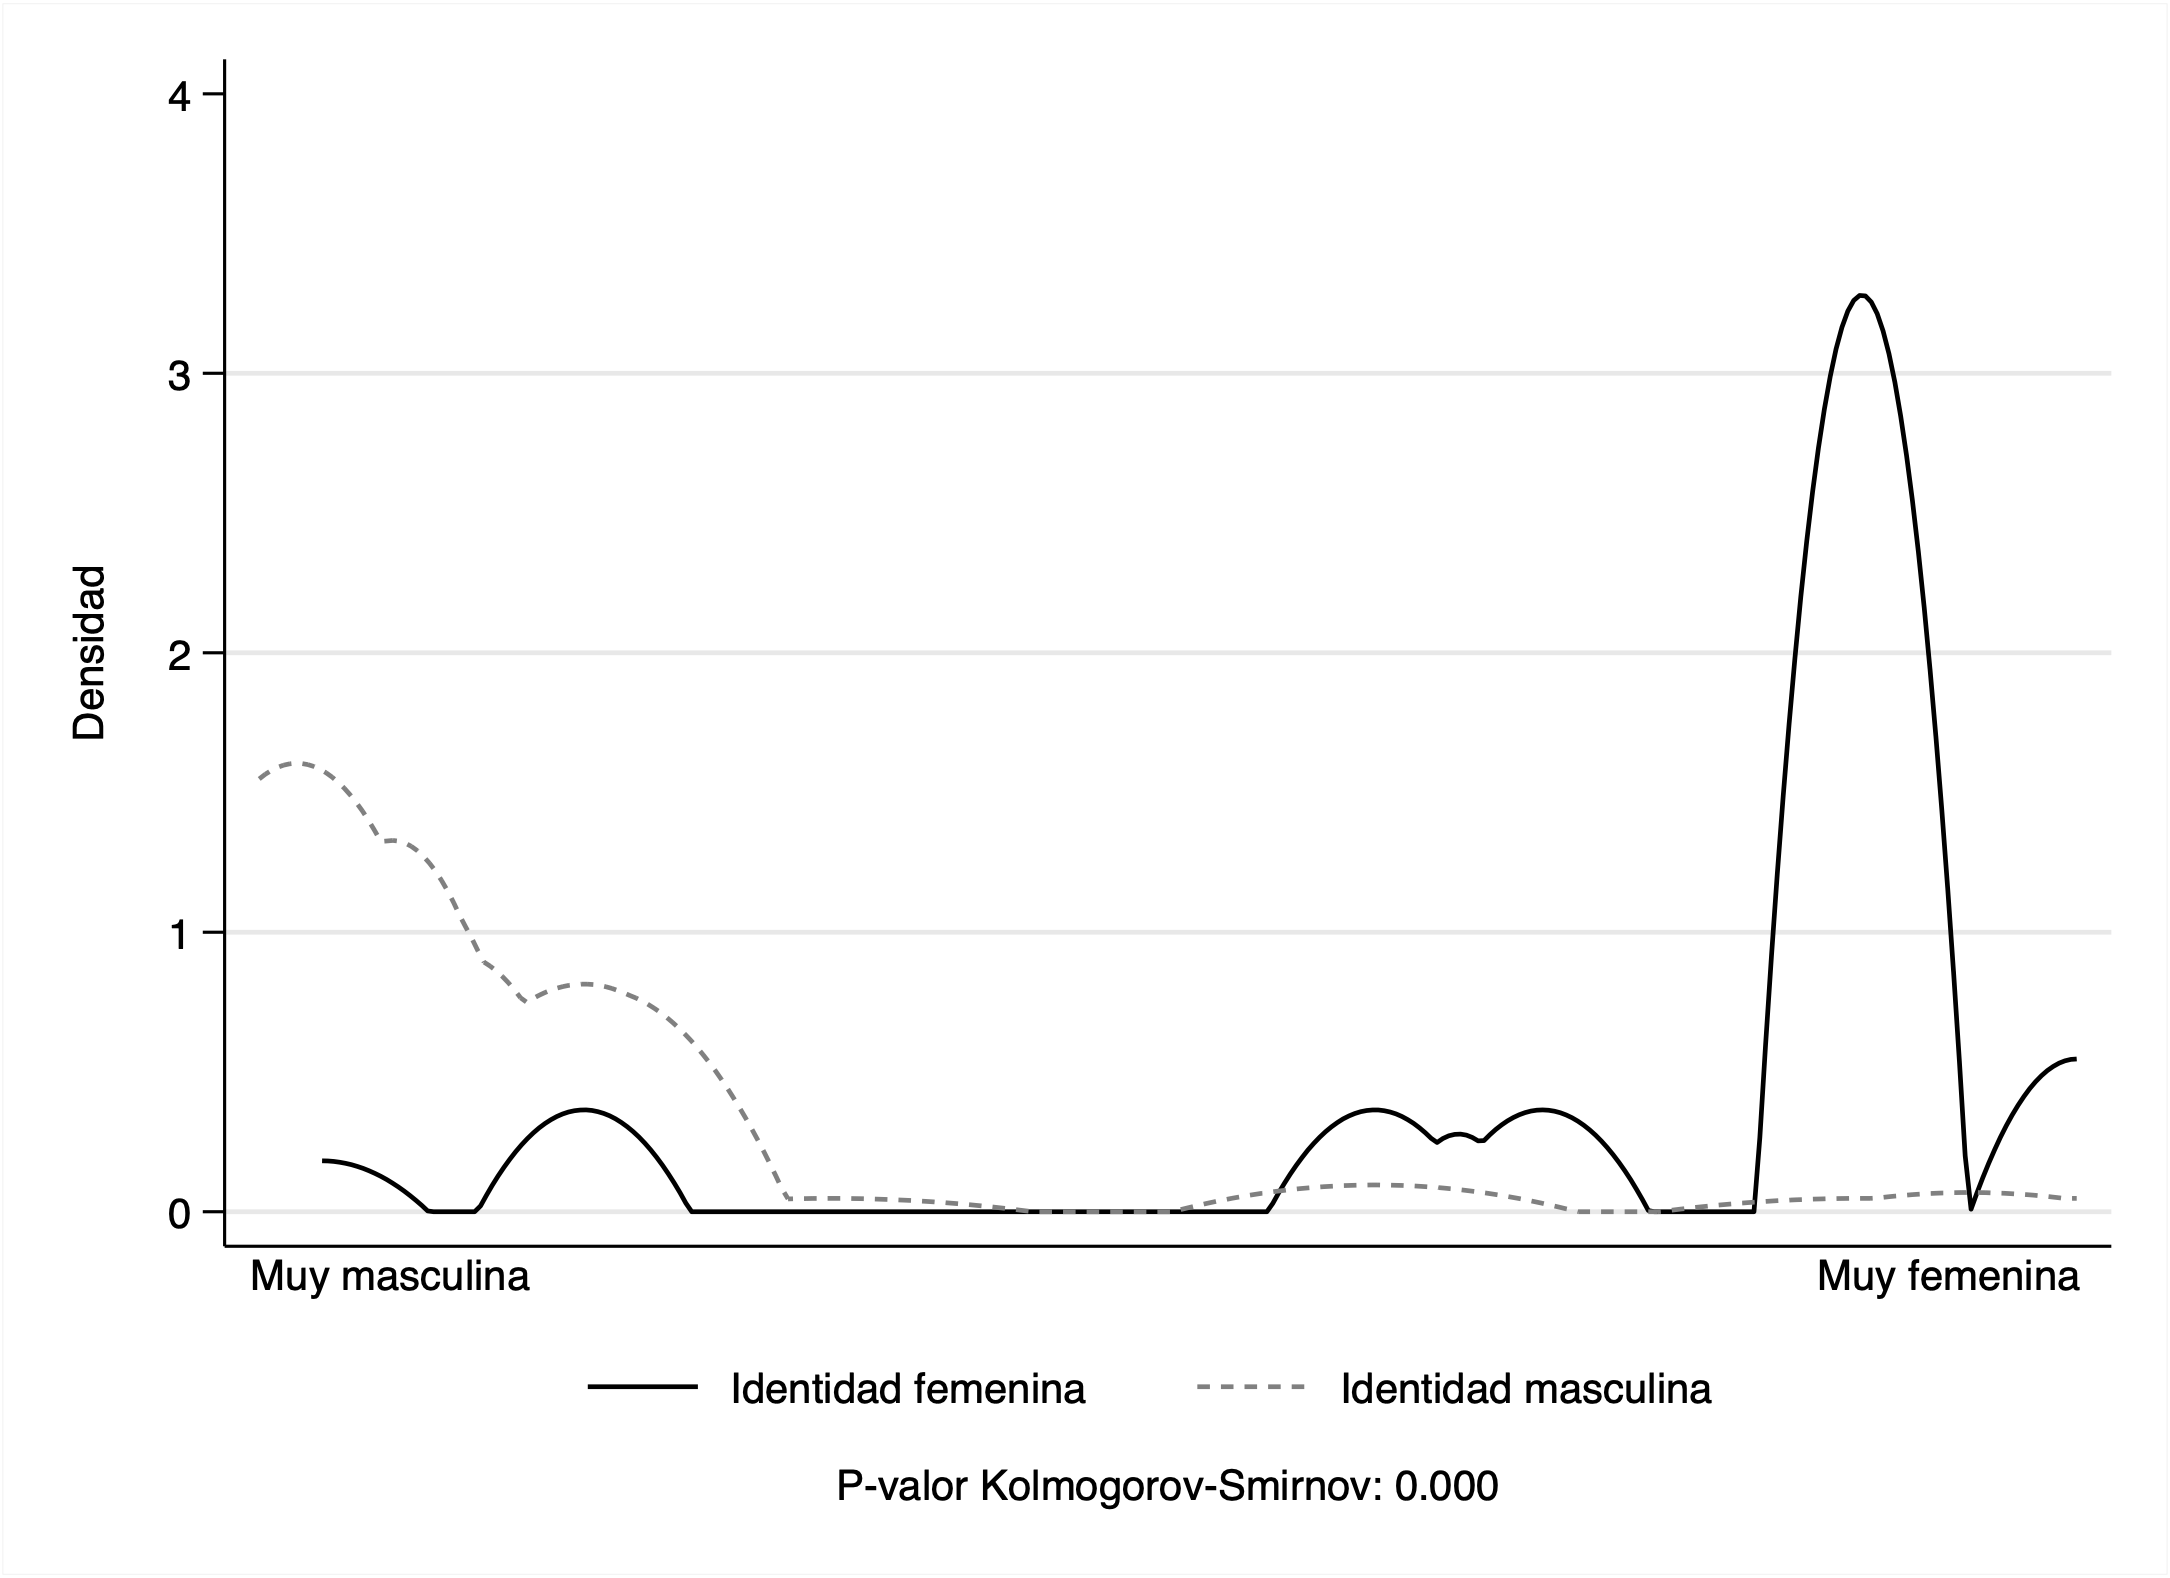
\includegraphics[width=13cm]{Images/dress_score_gender.png}
	\label{fig:dress_dist}
	\begin{singlespace}
    \floatfoot{\footnotesize{\textit{Nota:} Distribución del puntaje de vestimenta entre las vestimentas elegidas por los participantes del experimento. Prueba Kolmogorov-Smirnov de diferencia en la distribución por género.}\par}
    \end{singlespace}
\end{figure}
\begin{figure}[!ht]
	\centering
	\caption{Distribución habilidad}
	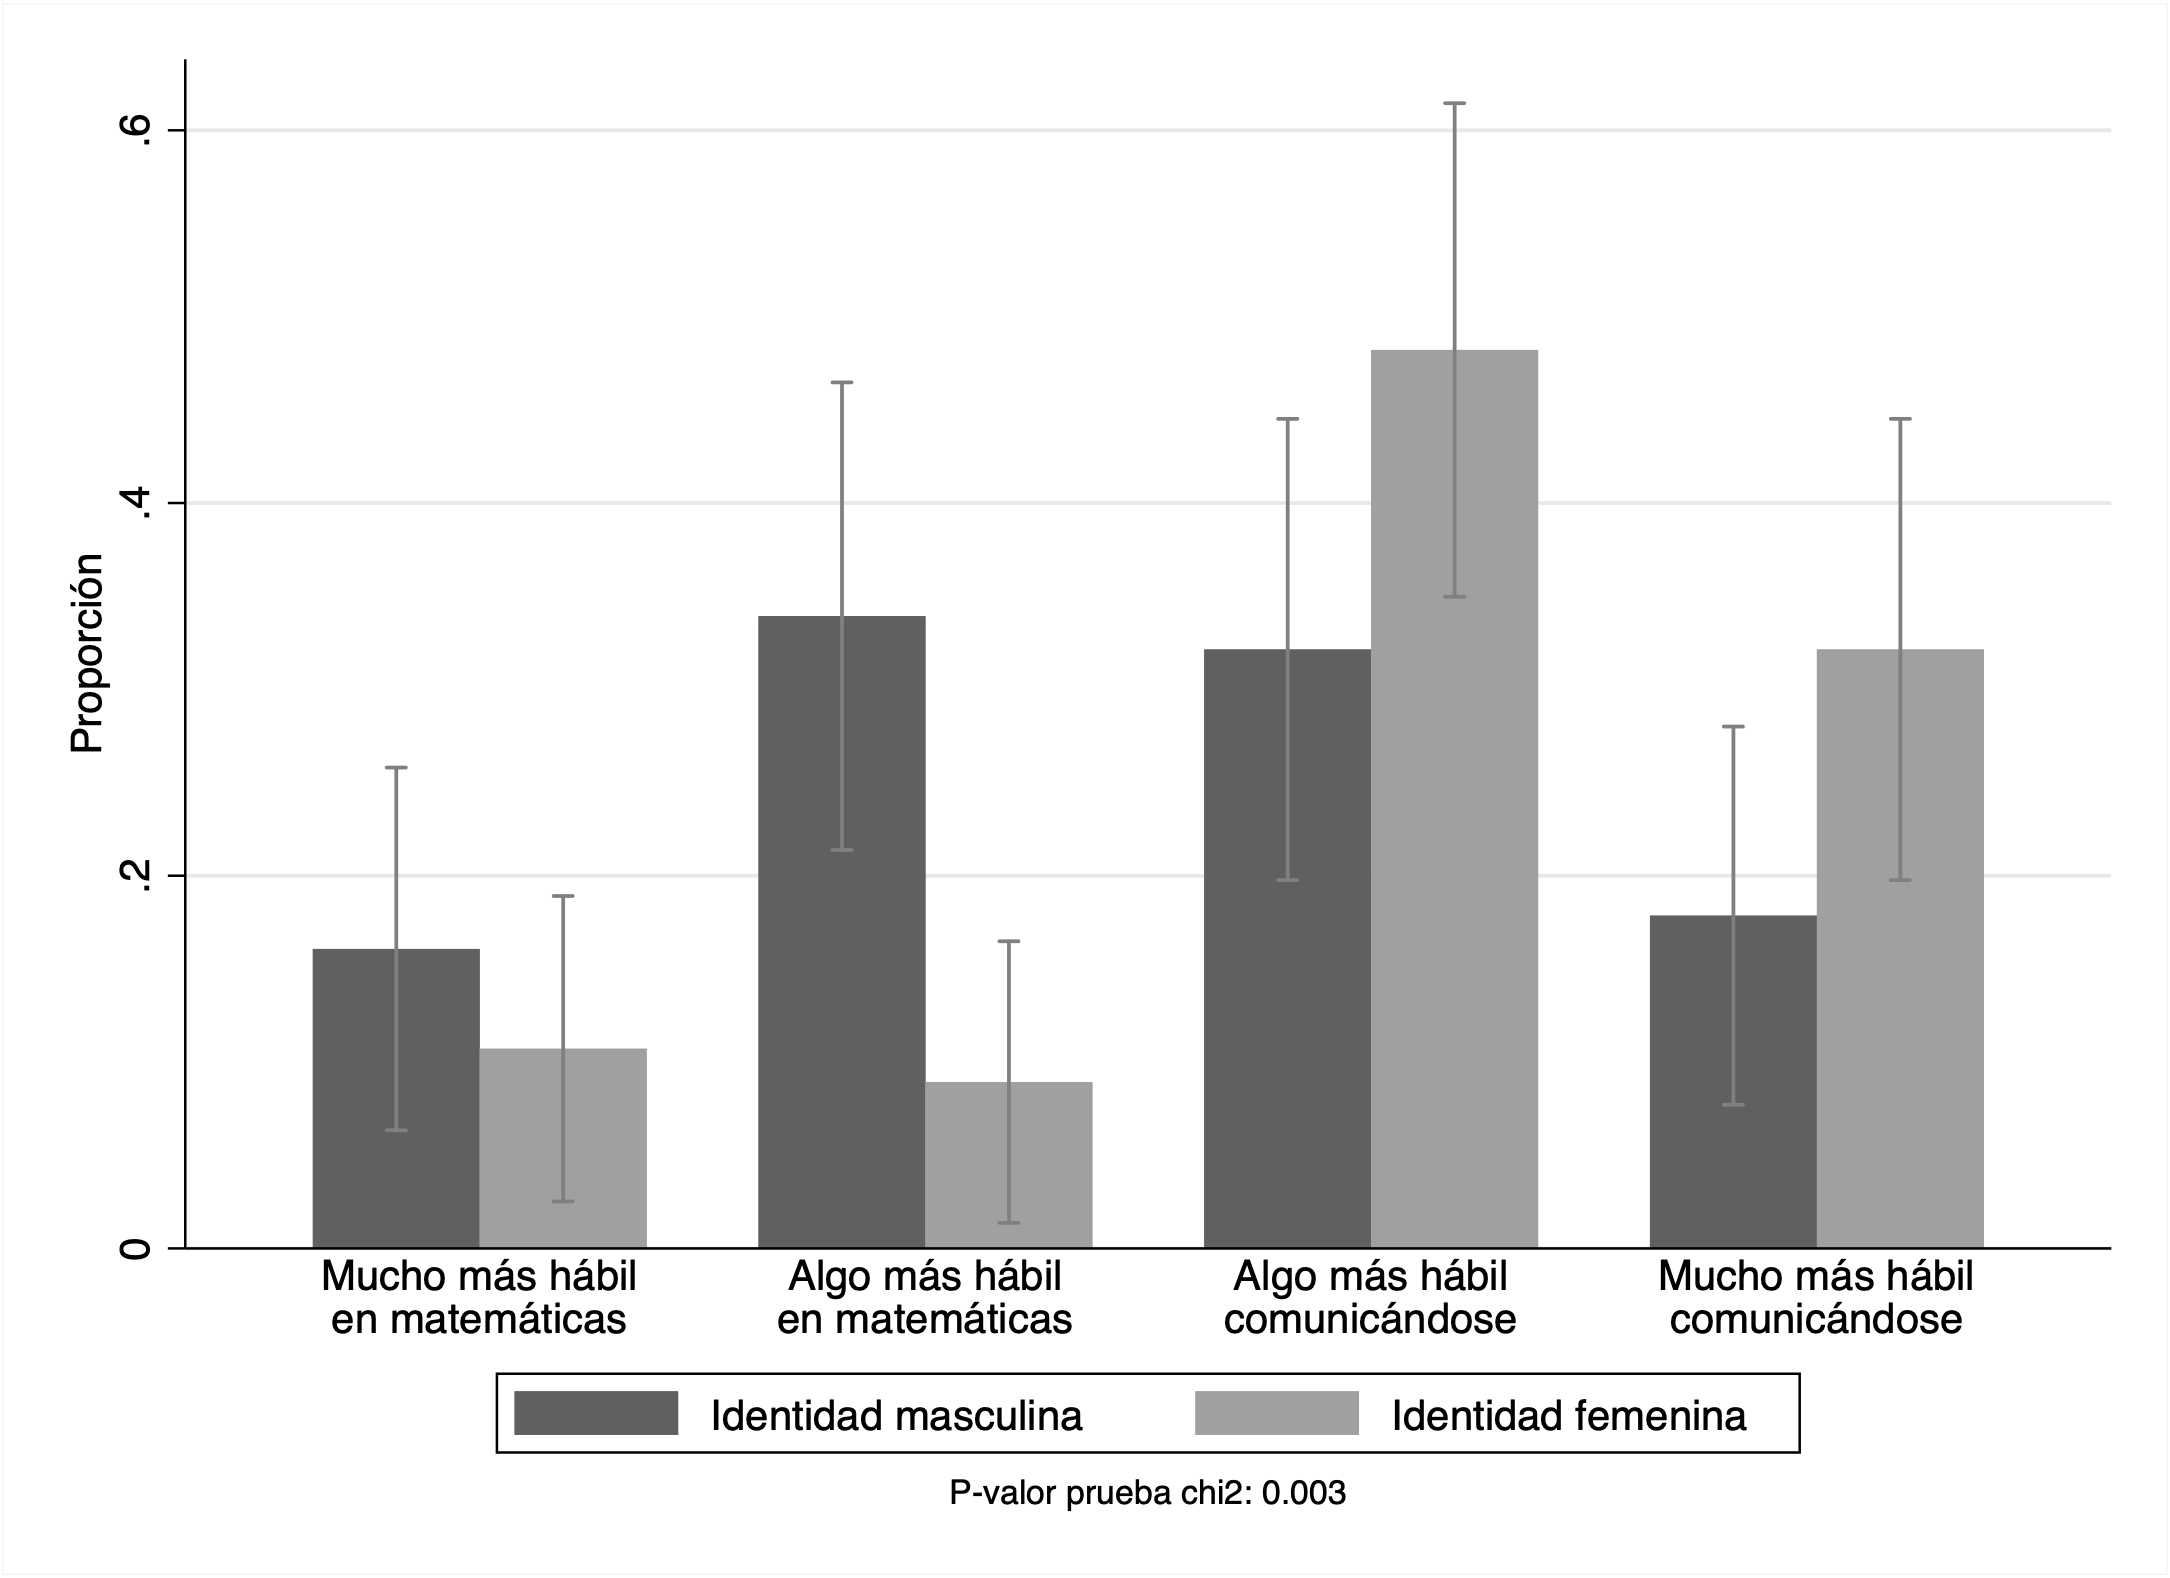
\includegraphics[width=12cm]{Images/ability_likert.png}
	\label{fig:ability_dist}
	\begin{singlespace}
    \floatfoot{\footnotesize{\textit{Nota:} Gráfica de respuestas de participante a la escala de likert sobre su principal habilidad, entre comunicación y matemáticas. Prueba chi2 de diferencia en género de indicador de si participante reportó ser más hábiles comunicándose que en matemáticas.}\par}
    \end{singlespace}
\end{figure}
\begin{figure}[!ht]
	\centering
	\caption{Distribución aspiraciones- reportada en escala de likert}
	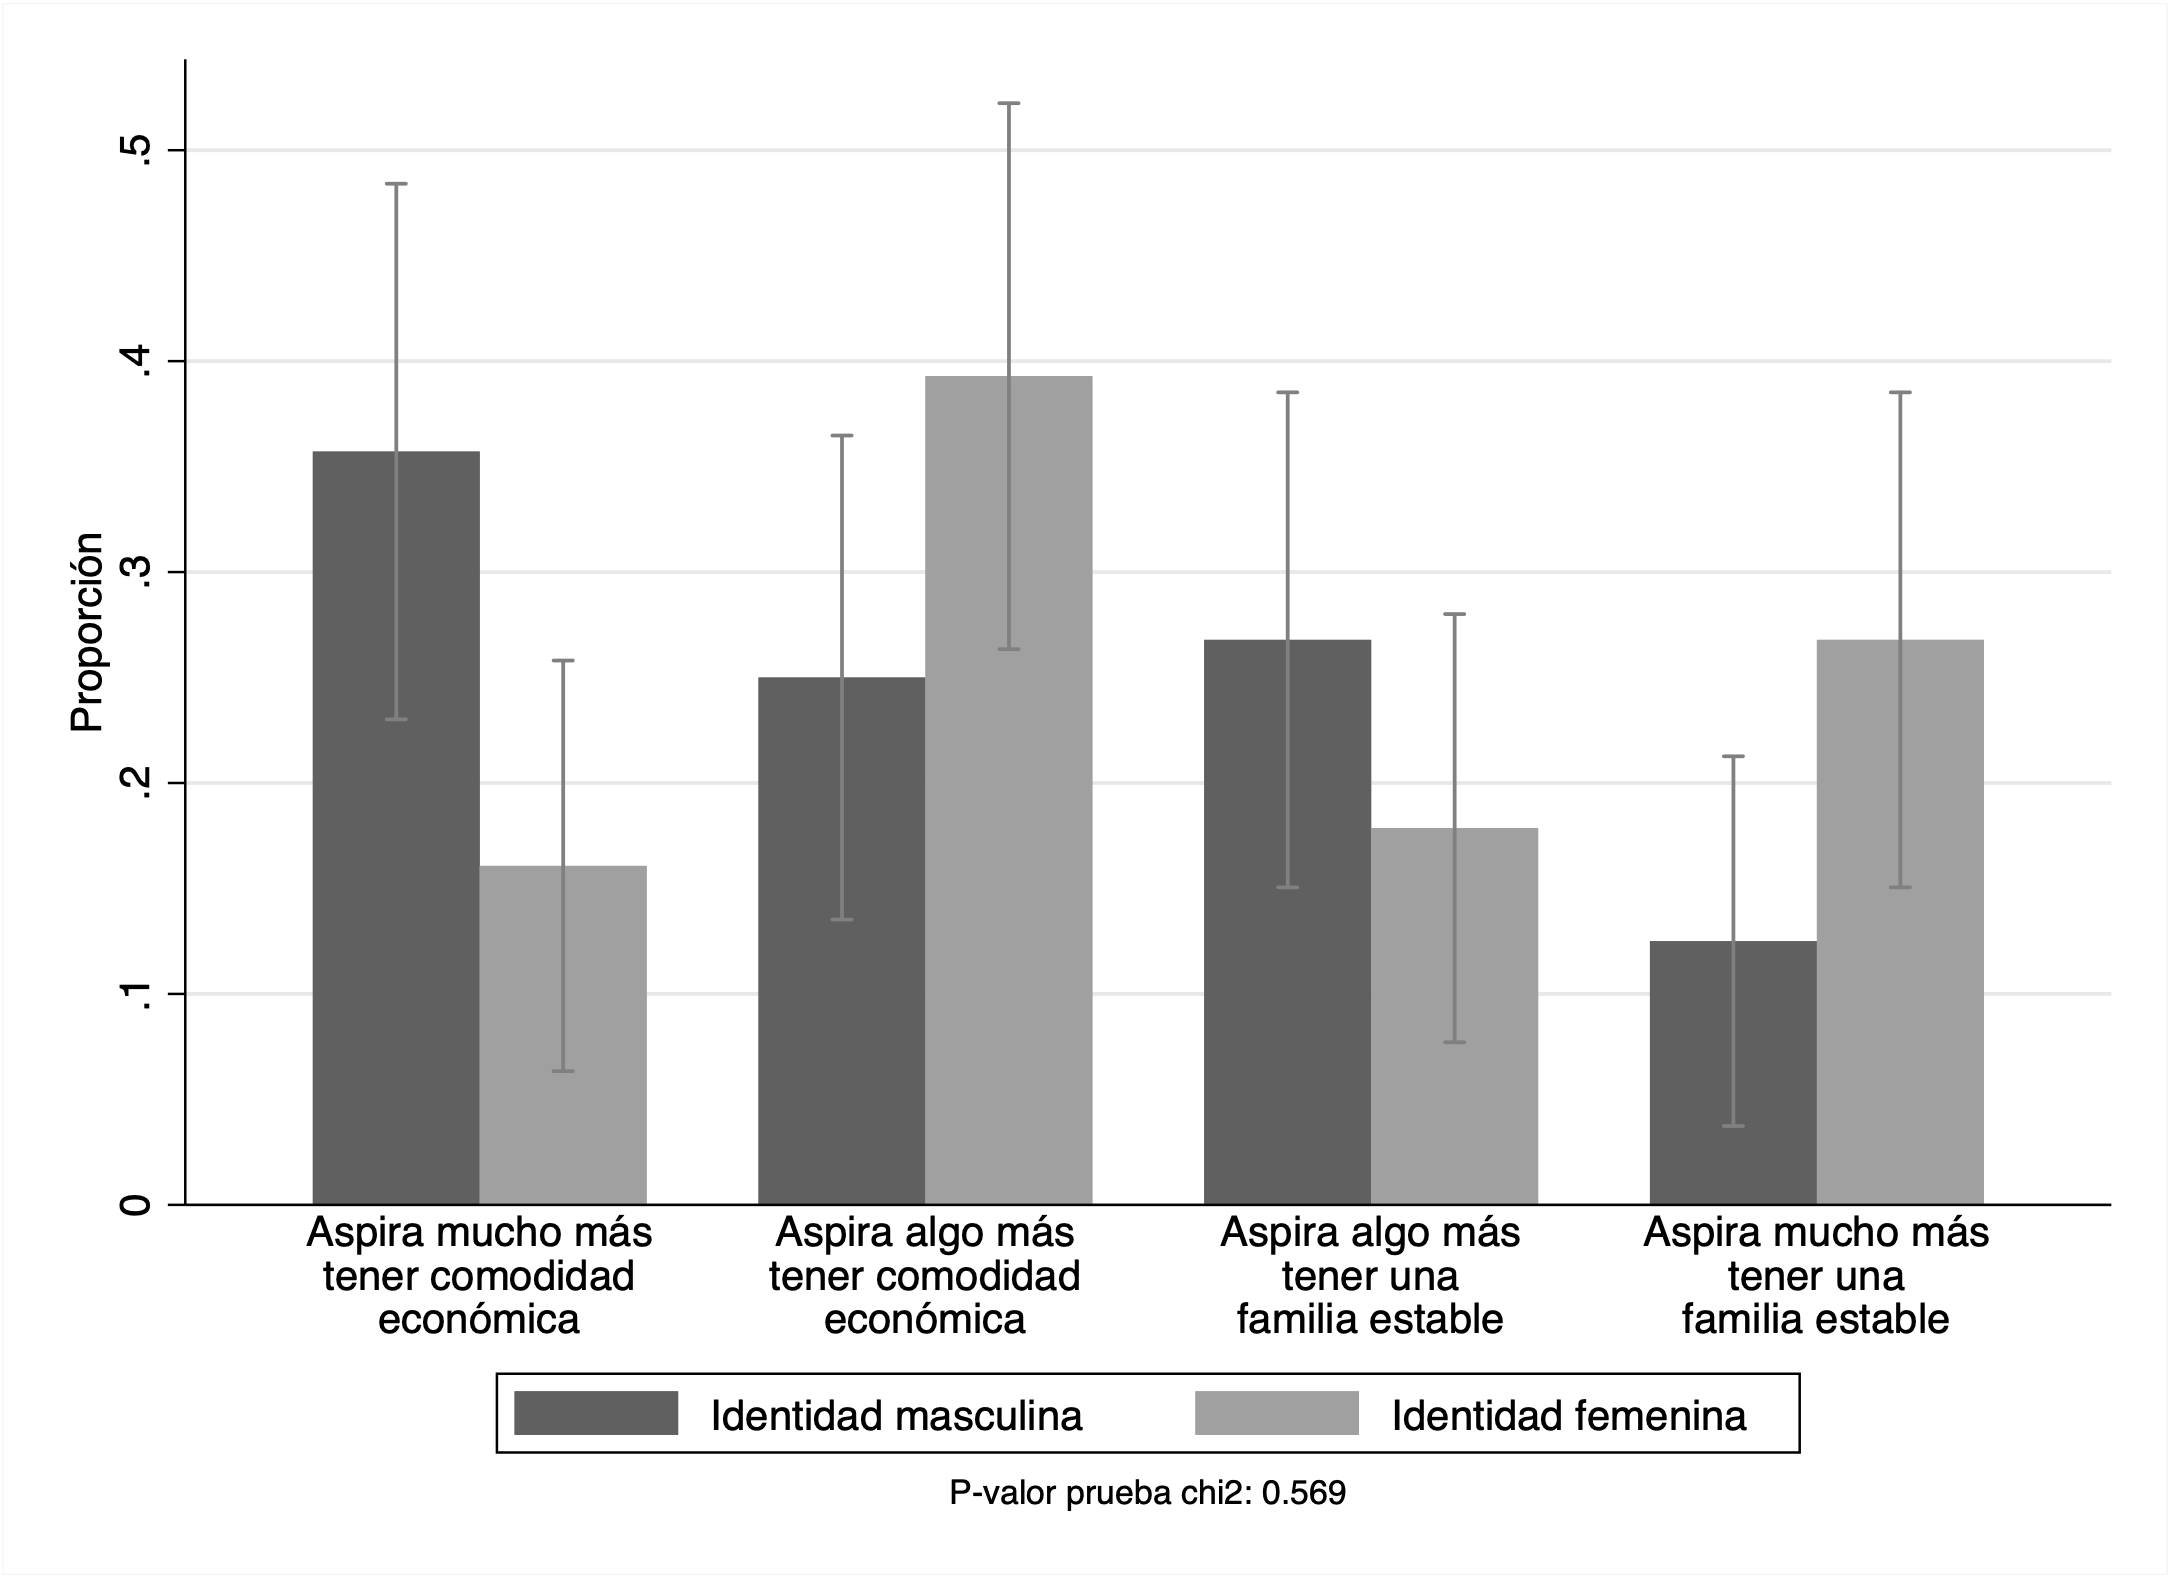
\includegraphics[width=12cm]{Images/aspiration_likert.png}
	\label{fig:aspiration_dist}
	\begin{singlespace}
    \floatfoot{\footnotesize{\textit{Nota:} Gráfica de respuestas de participante a la escala de likert sobre su aspiración principal, entre estabilidad familiar y estabilidad económica. Prueba chi2 de diferencia en género de indicador de si participante reportó aspirar más a tener estabilidad familiar que estabilidad económica.}\par}
    \end{singlespace}
\end{figure}
\begin{figure}[!ht]
	\centering
	\caption{Distribución de expresiones de género }
	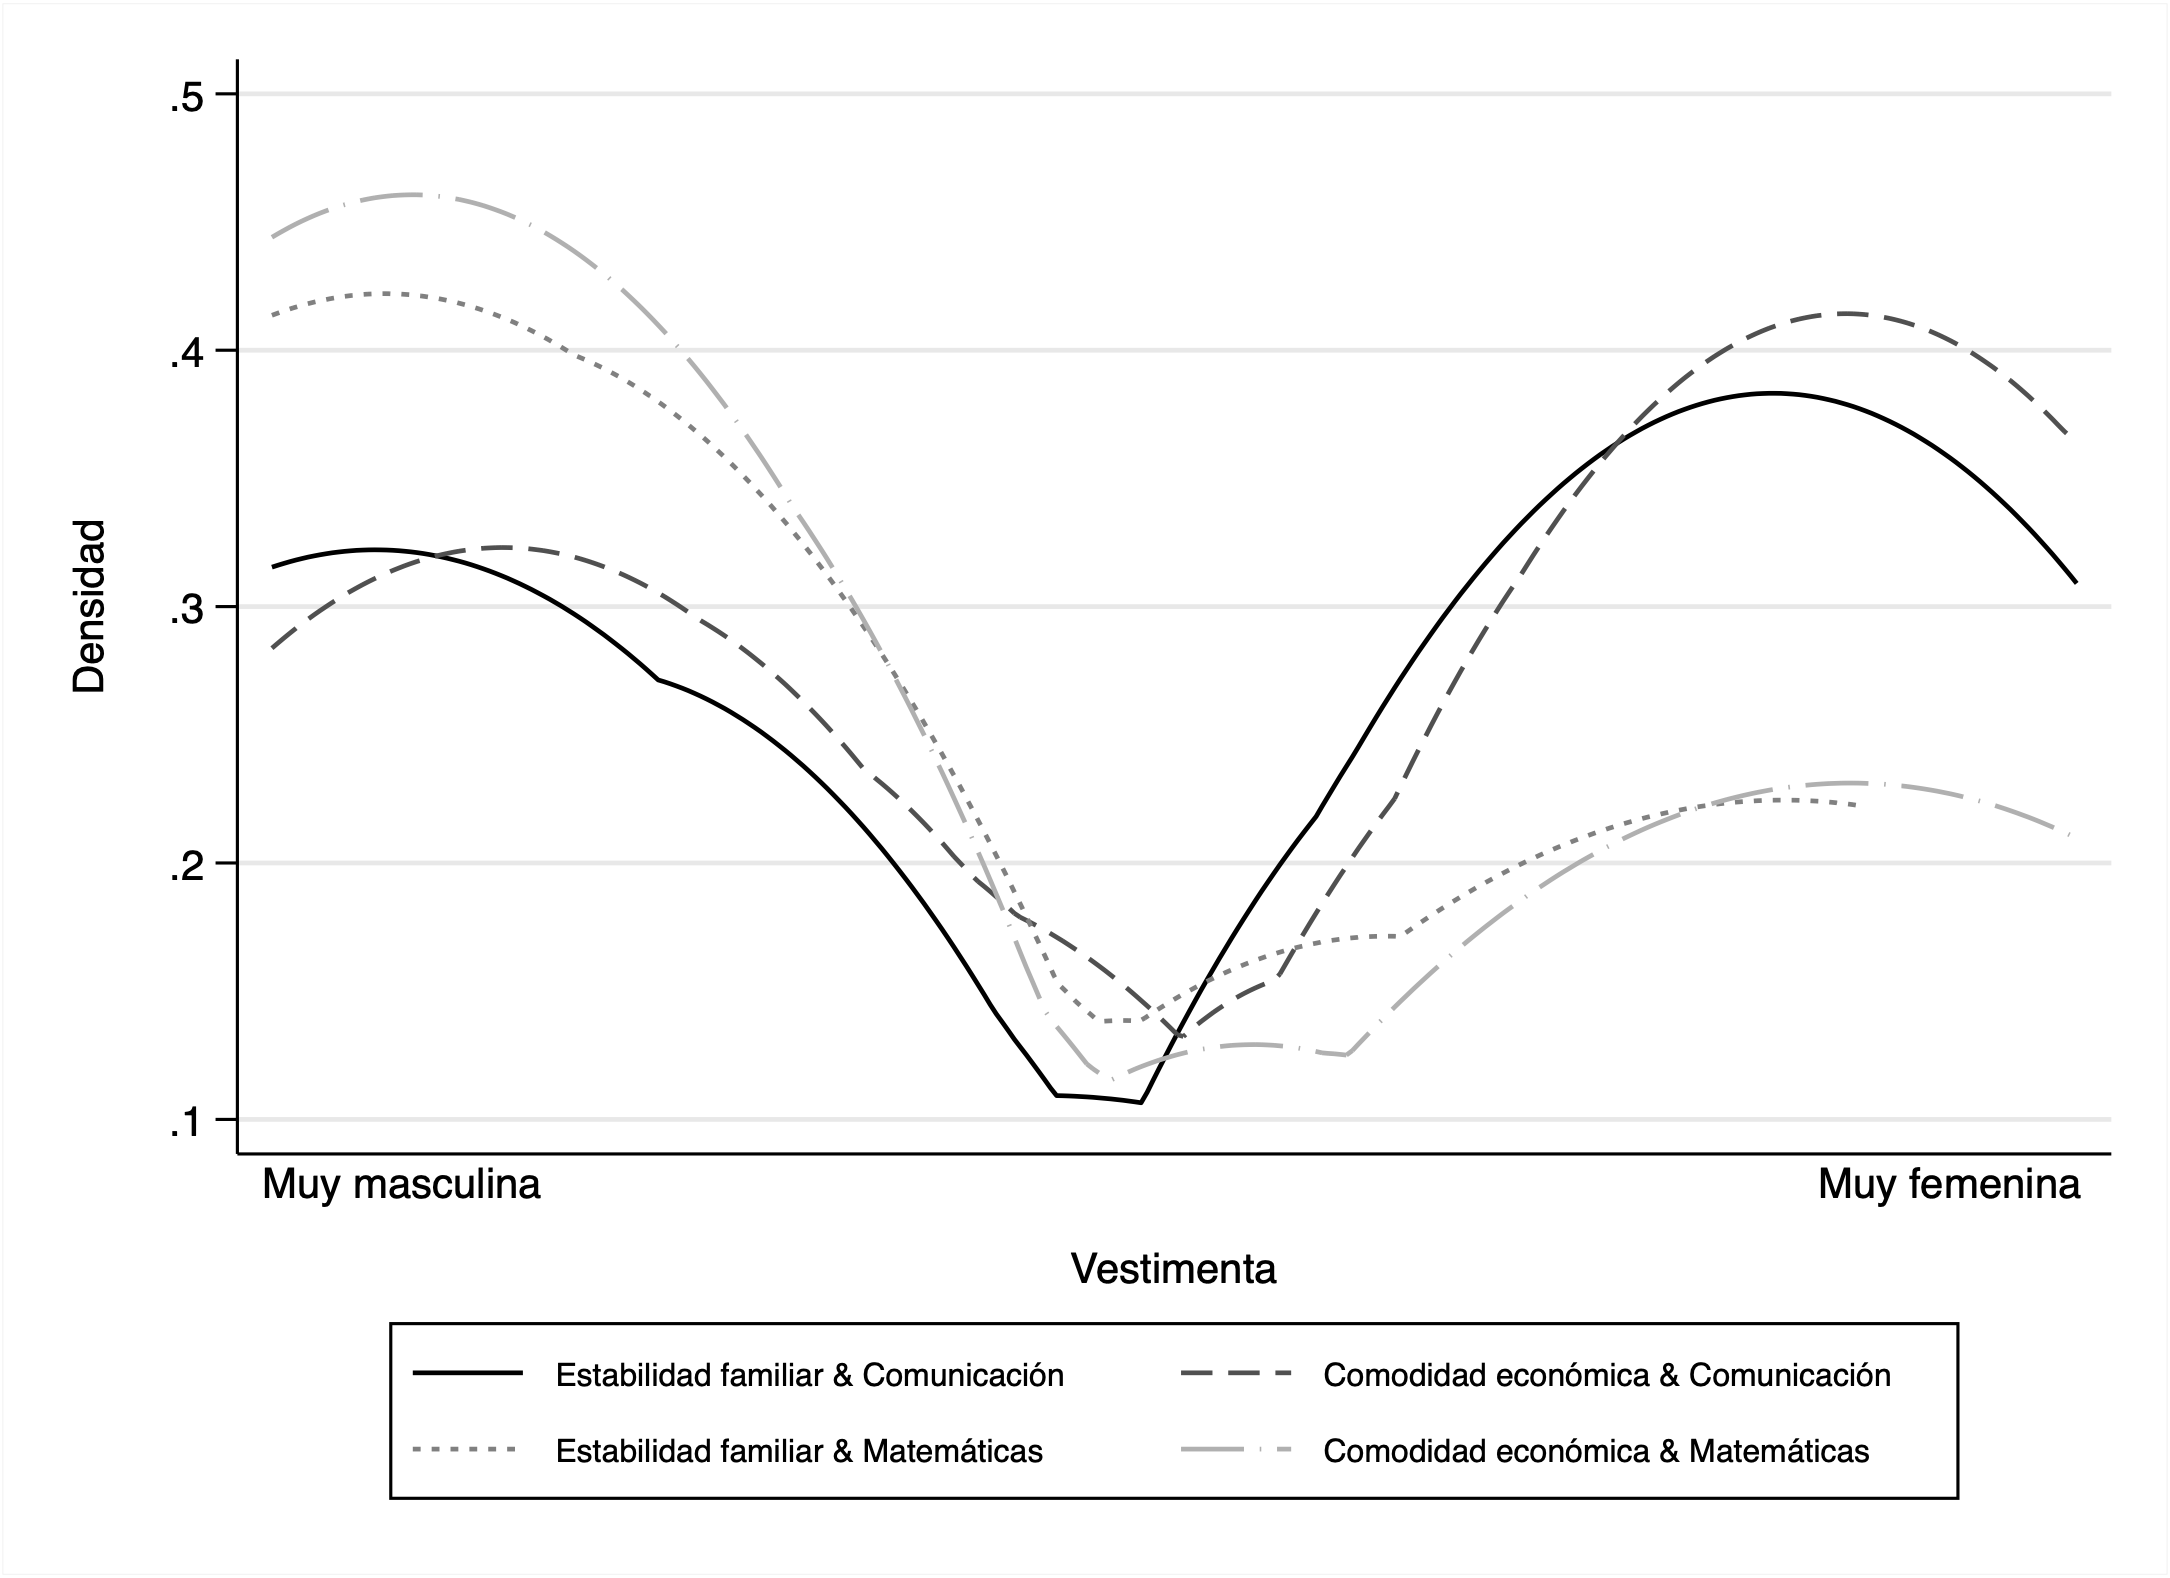
\includegraphics[width=12cm]{Images/gender_expressions.png}
	\label{fig:jointdistribution}
	\begin{singlespace}
    \floatfoot{\footnotesize{\textit{Nota:} Distribución por conjunto de expresiones de género.}\par}
    \end{singlespace}
\end{figure}
\vspace*{6cm}